\subsection {Session 9, Exercise 1}

\lineparagraph {Exercise}

Prove that the following languages are $NP$-complete.
\begin{enumerate}[a)]
    \item Language of those graphs that can be properly colored using $3$ colors, such that each color occurs
on the same number of vertices.
    \item Language of those quadruples $(G,a,b,k)$, where $G$ is an undirected graph, $a,b\in{}V(G)$ and $k > 0$
integer and there exists a path between vertices $a$ and $b$ of $G$ of length at least $k$.
    \item The language consisting of such triples $(G,a,b)$ that $G$ is an undirected graph $a,b > 0$ are integers
and $G$ an induced subgraph isomorphic to complete bipartite graph $K_{a,b}$.
    \item The language consisting of such undirected graphs $G$ that have a cycle $C$ such that every vertex $v \notin{} C$ is connected by an edge to a vertex of $C$.
\end{enumerate}

\lineparagraph {Solution}

\begin{itemize}
\item To prove that a language is $NP$-complete we must prove that it is both in $NP$ and $NP$-hard.
\item To prove that a language is in $NP$ we use the Witness Theorem.
\item To prove that a lanugage us $NP$-hard we find an already known $NP$-hard / $NP$-complete language and Karp-reduce this one onto the language in question, so we solve the well known $NP$-hard problem using the hypothetical solver for problem in question. E.g. $WellKnown \prec Question$.
\end{itemize}

\textbf{Task a):}

\begin{itemize}
    \item We first start with the Witness Theorem:
    \item The Witness will be the description of a $3$-coloring where each color occurs the same number of times. For $v$ vertices we can define an array $A[1:n]$ of numbers $1,2$ and $3$, where $A[i] = c$ means that the $i$th vertex has color $c$.
    \item The size of the Witness is polynomial relative to the input size, since the witness size is $2 bits \cdot{} n = O(n)$ (we can represent the $1,2,3$ numbers using $2$ bits), while the input size is $O(n^2)$ (the adjacency matrix of the graph).
    \item To check if this witness is a correct solution we check:
    \begin{itemize}
        \item The size of the array is the same as the number of vertices on the inputs.
        \item Only numbers $1,2$ and $3$ are present.
        \item We count the occurrences of the numbers and check that they are the same.
        \item We iterate through all edges of the graph and check that their ends don't have the same color, as that would be an improper coloring.
    \end{itemize}
    \item All these checks are iterating the vertices once or the edges once, so in total the runtime complexity is $O(n^2)$.
    \item Then we try to find a well-known NP-complete problem to Karp-reduce. You can find a table of all NP-complete problems we have studied in exercise \nameref{exam_2022_05_30_exercise_3}.
    \item It is a good idea to start with a similar problem and if it is not working out, then move on to others.
    \item In this case, $3-COLOR$ is a good choice to start with, since that is the most similar to our problem.
    \item So we are trying to give a $3-COLOR \prec L_a$ Karp-reduction: transform the input of $3-COLOR$ so that we can give it to the $L_a$ solver and it will correctly return $YES$ and $NO$.
    \item The solver of $L_a$ does almost what we need: but it additionally checks that the colors have to be assigned to the same number of vertices.
    \item We somehow want to skip this check, or make sure that it always succeeds.
    \item In the general $G$ graph input of $3-COLOR$, it is not necessarily true that the number of the $3$ colors will be equal, so we somehow want to transform $G$ to make sure that they are equal.
    \item We can do this by creating $3$ copies of the $G$ graph.
    \item If a proper $3$-coloring exists on $G$, then by creating $3$ copies, we allow the solver of $L_a$ to rotate the colors around the other $2$ copies of the $G$ graph, so in total it would assign one copy of each vertex red, one copy of each vertex blue and one copy of each vertex green, resulting in $n=n=n$ number of colors.
\end{itemize}

\begin{center}
    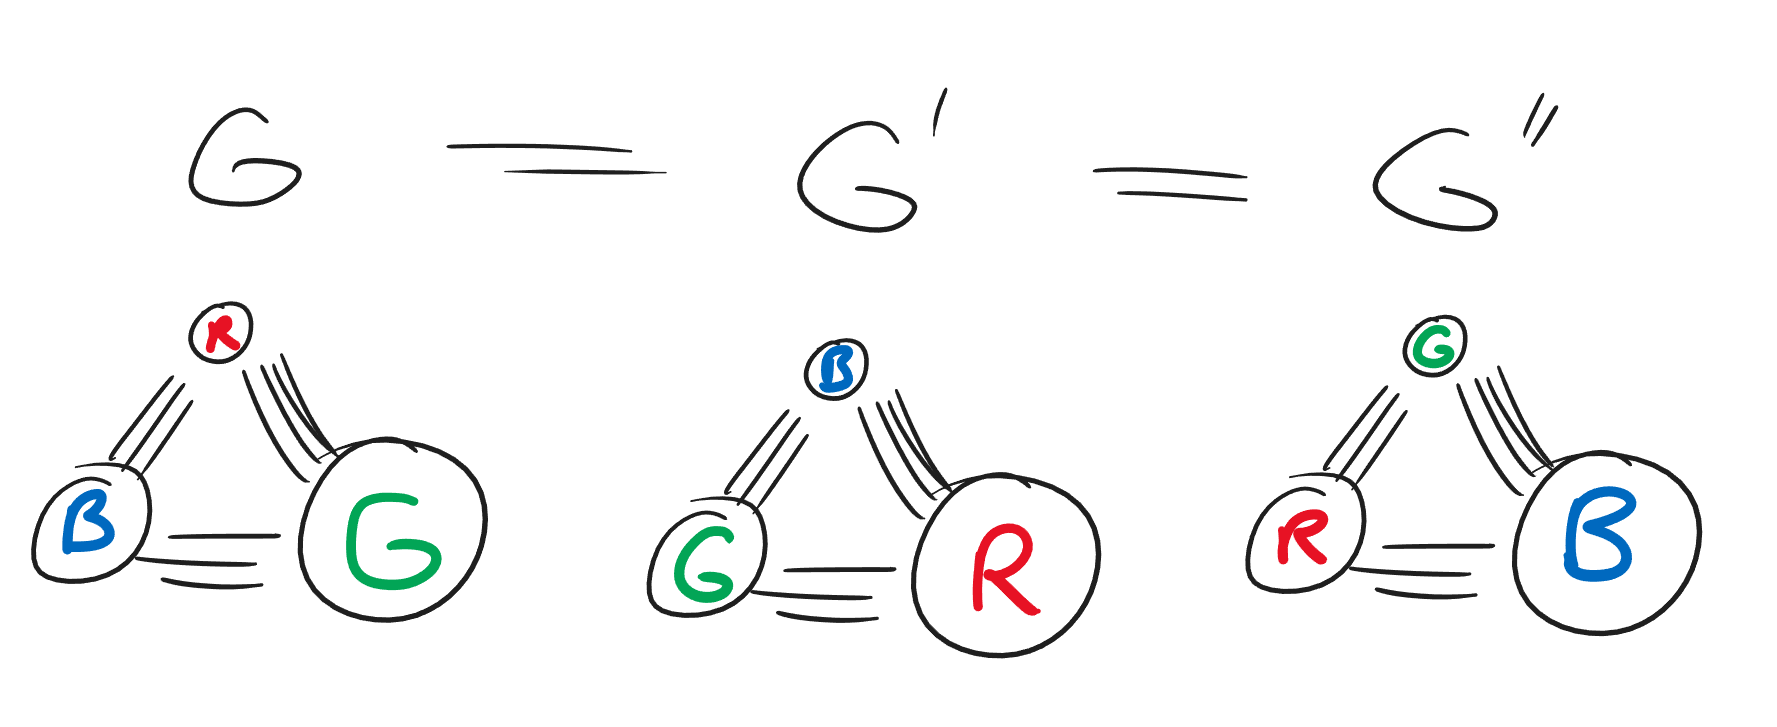
\includegraphics[width=\linewidth]{09/01/3_color_equal.png}
\end{center}

\begin{itemize}
    \item If no propert $3$ coloring exists, on the original $G$ graph, then there won't be any proper $3$ coloring on this new graph, since it contains $G$ three times.
    \item So with this modification, we are able to satisfy the one additional rule the $L_a$ solver is checking for and this makes sure that $L_a$ returns YES for the $f(G)$ graph exactly when for the $3-COLOR$ $G$ is a YES instance and NO when it's a NO instance.
    \item We can create a copy of $G$ 2 times in $O(n^2)$ time, by making the adjacency matrix $3$ times $3$ larger and copying the original one into it $3$ times.
    \item So $f$ also runs in polynomial time, which we need to check for a Karp-reduction.
\end{itemize}

\textbf{Task b)}:

\begin{itemize}
    \item Witness Theorem: The witness is the description of the undirected path in question, given by the list of vertices along it. Since a path has to have unique vertices along it, at most there will be $n$ vertices on the path and a single vertex can be given by it's index in binary format: $O(\log{}n)$ bits. So in total $O(n\log{}n)$ size, while the input is $O(n^2+\log_2(a)+\log_2(b)+\log_2(k))$, so it is polynomial.
    \item Witness Checking Algorithm: Chek if this is indeed at least $k$ vertices (and they are all indeed part of $G$) and that for all $v_i$ and $v_{i+1}$ vertex on the path, the edge exists between them in $G$. Also $v_1=a$ and the last $v_m=b$.
    \item We can Karp-reduce the $s-t-HAMPATH$ problem onto this. By assigning $k=n$, we require the path to be full length, of $n$ vertices, which is only possible if it is a Hamiltonian-path. Then, $a=s, b=t$ and the graph is the same. This transformation is trivially done in polynomial time.
\end{itemize}

\textbf{Task c)}:
\begin{itemize}
    \item Witness Theorem: The witness will be the list of vertices on side $A$ and side $B$ of the induced bipartite graph in question. This is similarly given in at most $O(\log{}n)$ bits, which is similarly polynomial as previously.
    \item Witness Checking Algorithm: Check all pairs of edges between vertices of $A$ and $B$, since we need a fully connected subgraph. Also check that there are no edges running inside $A$ and inside $B$ either, since the $K_{a,b}$ graph is induced, meaning that all edges present in the original graph must be part of it, so if $K_{a,b}$ is bipartite, it means that there are no edges running in $A$ and in $B$ either. This can be done in $O(n^2)$ time, so this is also polynomial. Check also that $|A|=a$ and $|B|=b$.
    \item Karp-reduction from well-known NP-complete problem: we can use the fact that $A$ and $B$ must be independent sets and Karp-reduce from $MAXINDEP$: $MAXINDEP \prec{} L_c$.
    \item We add $2$ additional vertices to the $G$ graph and connect both to all original vertices of $G$, but not to each other.
    \item Then, $MAXINDEP$'s input is $(G,k)$, where $k$ is the size of the independent set we are looking for. We can transform this into $(G', k, 2)$.
    \item If the $L_c$ solver finds such a $K_{k,2}$ bipartite graph, then it was either the $2$ vertices we just added, connected to a size $k$ independent set, or it might even find some induced subgraph completely in $G$ that meets the criteria. Either way, that will contain a size $k$ independent set for $|A|$, which is the correct solution to the original problem. If no such set exists, then $L_c$ won't find anything.
\end{itemize}

\begin{center}
    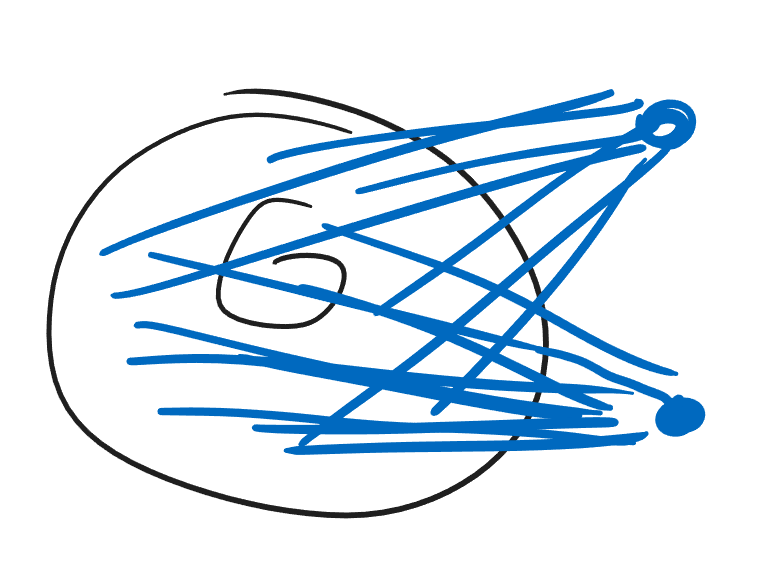
\includegraphics[width=\linewidth]{09/01/maxindep_karp.png}
\end{center}

\textbf{Task d)}:
\begin{itemize}
    \item Witness Theorem: The witness will be the description of this cycle in question. Given by the vertices of the cycle for example, in the order which they are encountered if we walked along the cycle. Similarly polynomial, size is $O(\log{}n)$ bits.
    \item Witness Checking Algorithm: Check that this is indeed a cycle, all edges exist between $v_i$ and $v_{i+1}$ neighbours, also $v_n$ and $v_1$. Check that the remaining vertices of the graph are all connected to one of the vertices of this cycle. This can be done by checking all edges at most, in $O(n^2)$ time. This is polynomial as well.
    \item Karp-reduction from well-known NP-complete problem: Let's use $HAM$, since that also has a cycle, the $HAM$ cycle. We want our solver to find a $HAM$ cycle. However the solver allows these dangling vertices as well. We want to modify our original input graph, such that all original vertices must be present in the cycle the solver finds. We can do this by adding $n$ extra vertices to graph $G$, the $i$th connected to the original $i$th vertex of $G$.
    \item The blue vertices can never be part of the cycle found, since they only have a single edge. So they all will be dangling. This means that their neighbour must be part of the cycle, making all original vertices a must for the cycle that the $L_d$ solver finds. This means that the $L_d$ solver will find a HAM-cycle if it exist, and won't find anything if it doesn't.
    \item Adding $n$ vertices to $G$ and $n$ corresponding edges can also be done in polynomial time.
\end{itemize}

\begin{center}
    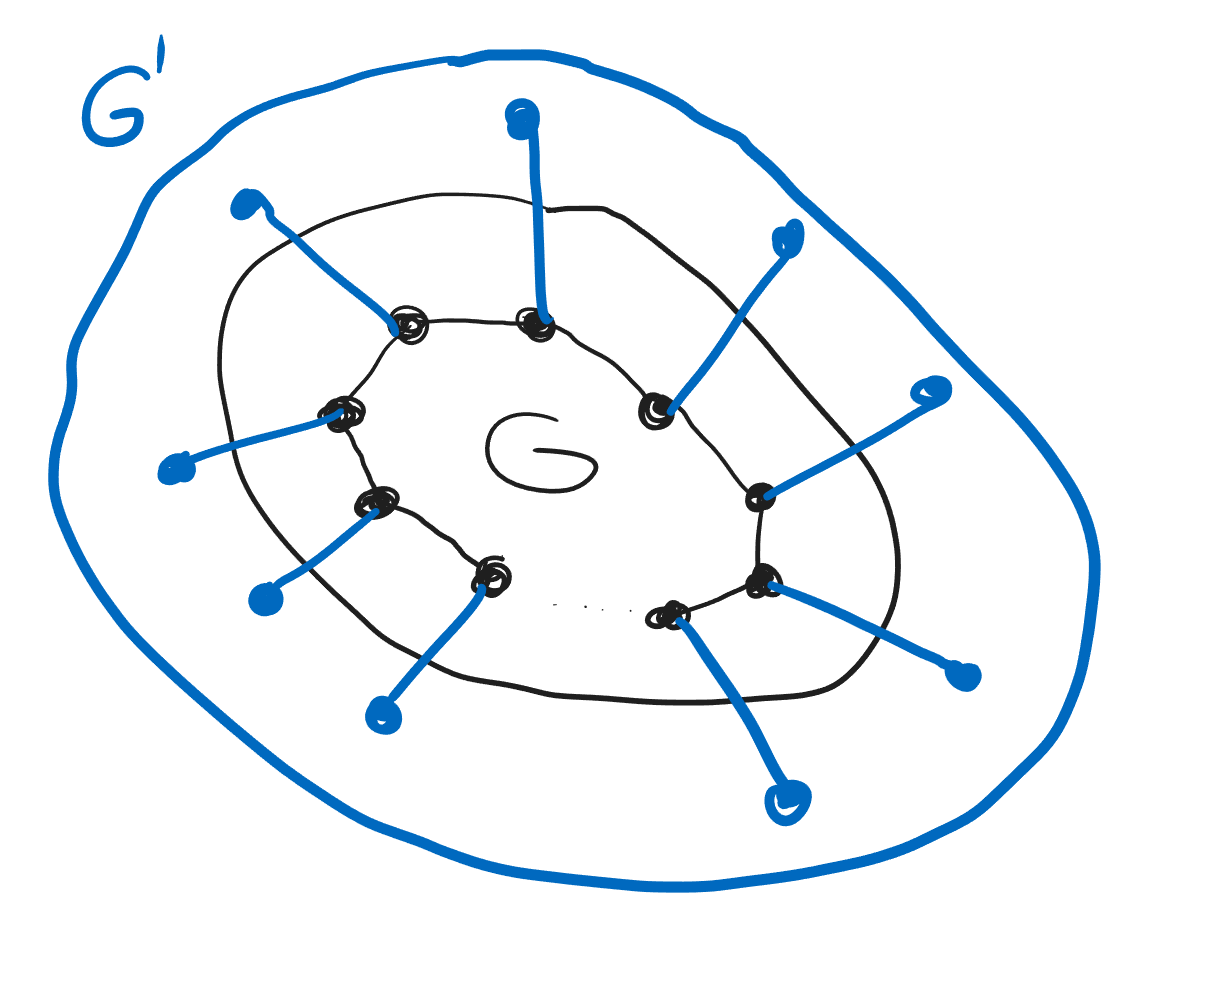
\includegraphics[width=\linewidth]{09/01/ham_karp.png}
\end{center}